\hypertarget{architecture-styles-architecture-patterns}{%
\section{Architecture Styles, Architecture
Patterns}\label{architecture-styles-architecture-patterns}}

\begin{tcolorbox}[colback=blue!5!white,colframe=blue!75!black]
\begin{itemize}
    \item You’ll learn what the terms “style” and “pattern” mean
    \item You’ll familiarize yourself with some (important) architecture styles and patterns
\end{itemize}
\end{tcolorbox}


\textbf{Architectural style}:\\
Set of established architectural organizations, components,
relationships, connectors, \ldots{}

\textbf{Two categories of ``Architectural Styles''}:

\begin{itemize}
\tightlist
\item
  Patterns

  \begin{itemize}
  \tightlist
  \item
    Includes well-known organizational structures such as

    \begin{itemize}
    \tightlist
    \item
      layered systems, pipes and filters, etc.
    \end{itemize}
  \end{itemize}
\item
  Reference Models

  \begin{itemize}
  \tightlist
  \item
    Prescribes specific configurations of components and interactions
    {[}\ldots{}{]}.
  \end{itemize}
\end{itemize}

\hypertarget{patterns-in-general}{%
\subsection{Patterns in general}\label{patterns-in-general}}

\begin{itemize}
\tightlist
\item
  Descriptions of successful engineering stories
\item
  Address recurring problems
\item
  Describe generic solutions that worked
\end{itemize}

\textbf{Design Patterns}:\\
Scheme for refining subsystems or components. Commonly recurring
structure of communication components that solves a general design
problem within a particular context {[}GOF{]}

\hypertarget{strategy-pattern-example}{%
\subsubsection{Strategy Pattern
Example}\label{strategy-pattern-example}}

\begin{figure}[H]
\centering
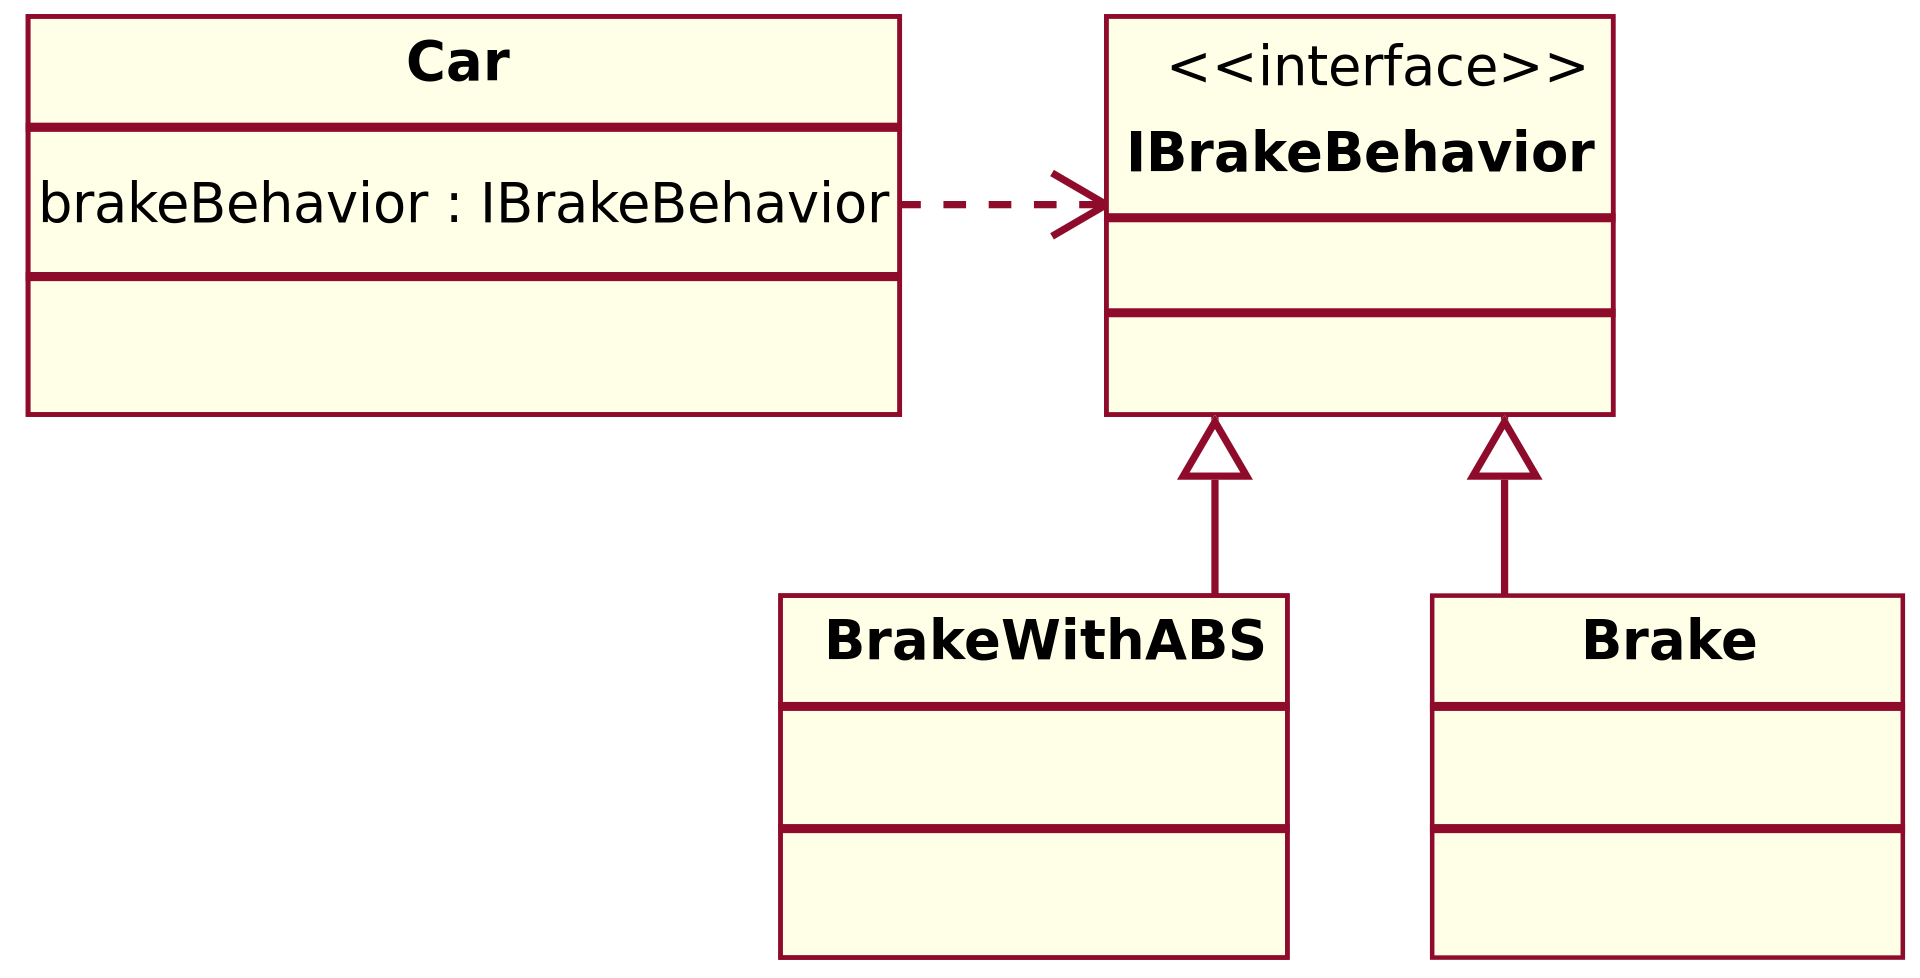
\includegraphics[width=0.5\textwidth]{figures/StrategyPattern_IBrakeBehavior.png}
\caption{Strategy Pattern}
\end{figure}

\hypertarget{decorator-pattern-example}{%
\subsubsection{Decorator Pattern
Example}\label{decorator-pattern-example}}

\begin{figure}[H]
\centering
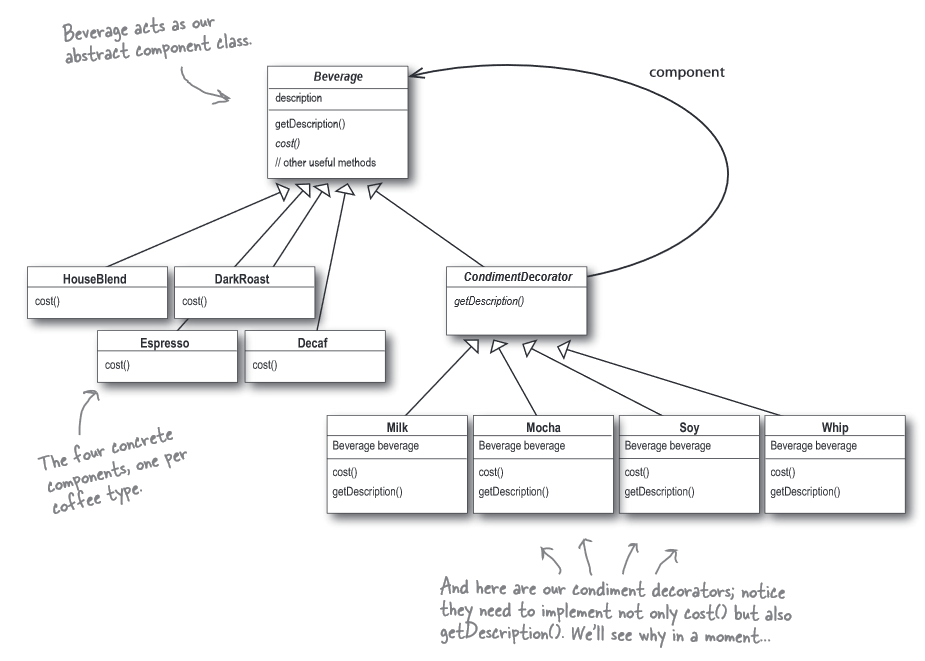
\includegraphics[width=0.5\textwidth]{figures/decorator_pattern.png}
\caption{Decorator Pattern}
\end{figure}

The decorator decorates (wraps) objects. It is able to add dynamically object to another object etc. The method calls are delegated to the next inner instances and so on. 
\begin{itemize}
    \item Advantages
    \subitem Flexbility and Dynamic, Robustness and Scalability also Consitency and Mainainability!
    \item Disadvantages
    \subitem Hard to find bugs, Komplexity, no objectidentity
\end{itemize}

\begin{lstlisting}
public static void main(String[] args) { 
    Beverage drink = new Mocha(new DarkRoast()); 
    drink.getDescription(); 
    //DarkRoast, Mocha 
    System.out.println(" fuer "+drink.cost() + " CHF"); 
    // fuer 9 CHF 
    
    drink = new Whip(drink); 
    drink.getDescription();
    //DarkRoast, Mocha , Whip
    System.out.println(" fuer "+drink.cost() + " CHF"); 
    // fuer 11 CHF 
} 
\end{lstlisting}






\hypertarget{architecture-styles-and-patterns}{%
\subsection{Architecture styles and
patterns}\label{architecture-styles-and-patterns}}

\begin{tcolorbox}[colback=red!5!white,colframe=red!75!black]
A pattern for software architecture describes a particular
recurring design problem that arises in specific design contexts, and
presents a well-proven generic scheme for its solution.
\end{tcolorbox}

\hypertarget{layers}{%
\subsubsection{Layers}\label{layers}}

The Layers architectural pattern helps to structure applications that
can be decomposed into groups of subtasks in which each group of
subtasks is at a particular level of abstraction

e.g.~View, Model, Controller or the TCP stack

\hypertarget{pipes-and-filters}{%
\subsubsection{Pipes and Filters}\label{pipes-and-filters}}

\begin{itemize}
\tightlist
\item
  Structure for systems that process a stream of data
\item
  Each step is encapsulated in a filter
\item
  Data is passed through pipes (connectors) between adjacent filters

  \begin{itemize}
  \tightlist
  \item
    Buffering
  \item
    Sychronisation
  \end{itemize}
\end{itemize}

\begin{figure}[H]
\centering
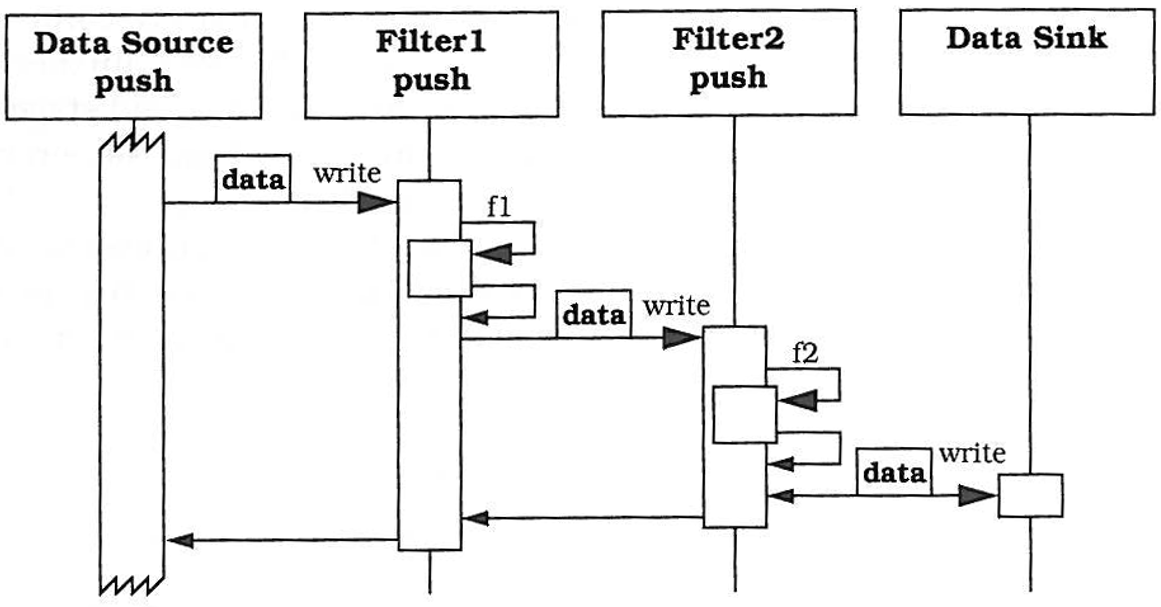
\includegraphics[width=0.5\textwidth]{figures/pipepush.png}
\caption{Pipe Push}
\end{figure}

\begin{figure}[H]
\centering
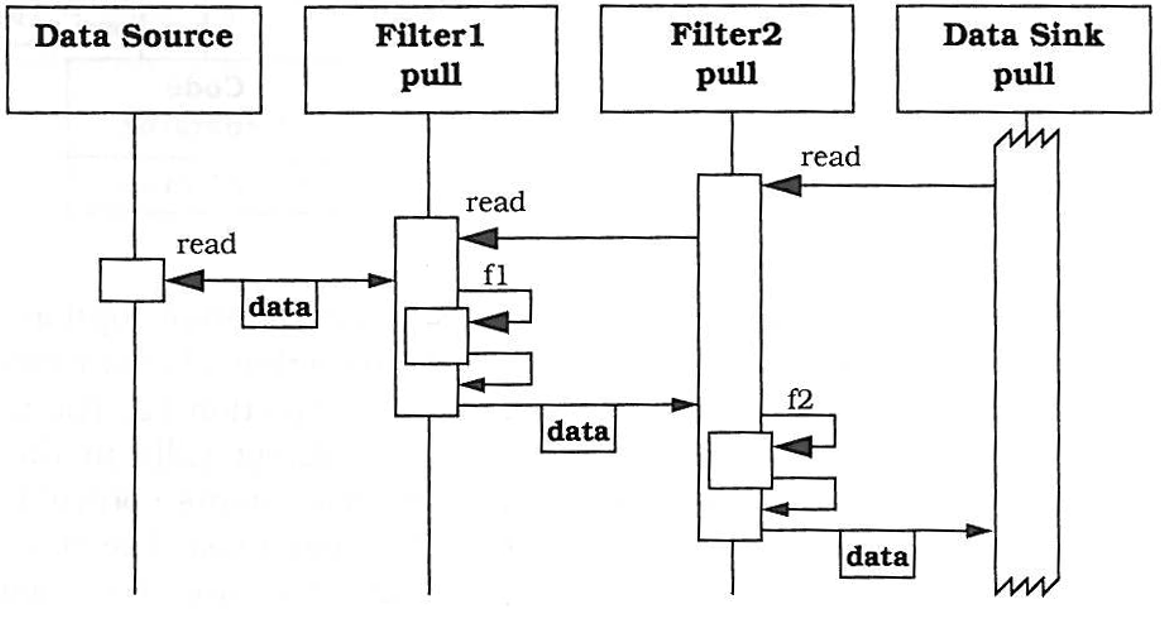
\includegraphics[width=0.5\textwidth]{figures/pipepull.png}
\caption{Pipe Pull}
\end{figure}

\hypertarget{blackboard}{%
\subsubsection{Blackboard}\label{blackboard}}

\begin{itemize}
\tightlist
\item
  Blackboard as common exchange of information
\item
  subsystems that process the available information and produce (and
  publish) new ones
\item
  control component that orchestrates the subsystems
\end{itemize}

\hypertarget{ways-of-integrating-enterprise-applications}{%
\subsubsection{Ways of integrating enterprise
applications}\label{ways-of-integrating-enterprise-applications}}

\begin{itemize}
\tightlist
\item
  (Shared) Database
\item
  File-based
\item
  Remote Procedure Invocation
\item
  Messaging
\end{itemize}


\hypertarget{dangers-of-patterns}{%
\subsubsection{Dangers of Patterns}\label{dangers-of-patterns}}

\begin{itemize}
\tightlist
\item
  Too much flexibility

  \begin{itemize}
  \tightlist
  \item
    think about YAGNI and Simple Code!
  \end{itemize}
\item
  Too many patterns in a design

  \begin{itemize}
  \tightlist
  \item
    use where you really have the problem and can live with the
    drawbacks!
  \end{itemize}
\item
  separate patterns split into separate classes

  \begin{itemize}
  \tightlist
  \item
    typical beginners' mistake !
  \item
    class explosion
  \end{itemize}
\item
  Over-engineering
\item
  Misunderstanding the example/diagram for the pattern
\end{itemize}

\hypertarget{things-to-know}{%
\subsubsection{Things to know}\label{things-to-know}}

\begin{itemize}
\tightlist
\item
  There are more than 23 patterns
\item
  Pattern names give us a common vocabulary to discuss design
  efficiently

  \begin{itemize}
  \tightlist
  \item
    Alternatives
  \item
    Higher-level abstractions of object interactions
  \item
    Architectures
  \end{itemize}
\item
  A pattern names a recurring successful solution concept
\item
  Honest pattern descriptions tell drawbacks and alternatives
\item
  Patterns are targets for refactoring!
\item
  Beware of YAGNI ! Create simple code!
\end{itemize}




\subsection{Model-View-Controller}
\begin{itemize}
    \item Model
    \subitem It Contains the Data which will be represented in the View. Also is open for changes by the controller.
    \item View
    \subitem Presents the Data. It is Connected to the Model because it fetches the data there.
    \item Controller
    \subitem Controlls the data. 
\end{itemize}

\begin{figure}[H]
\centering
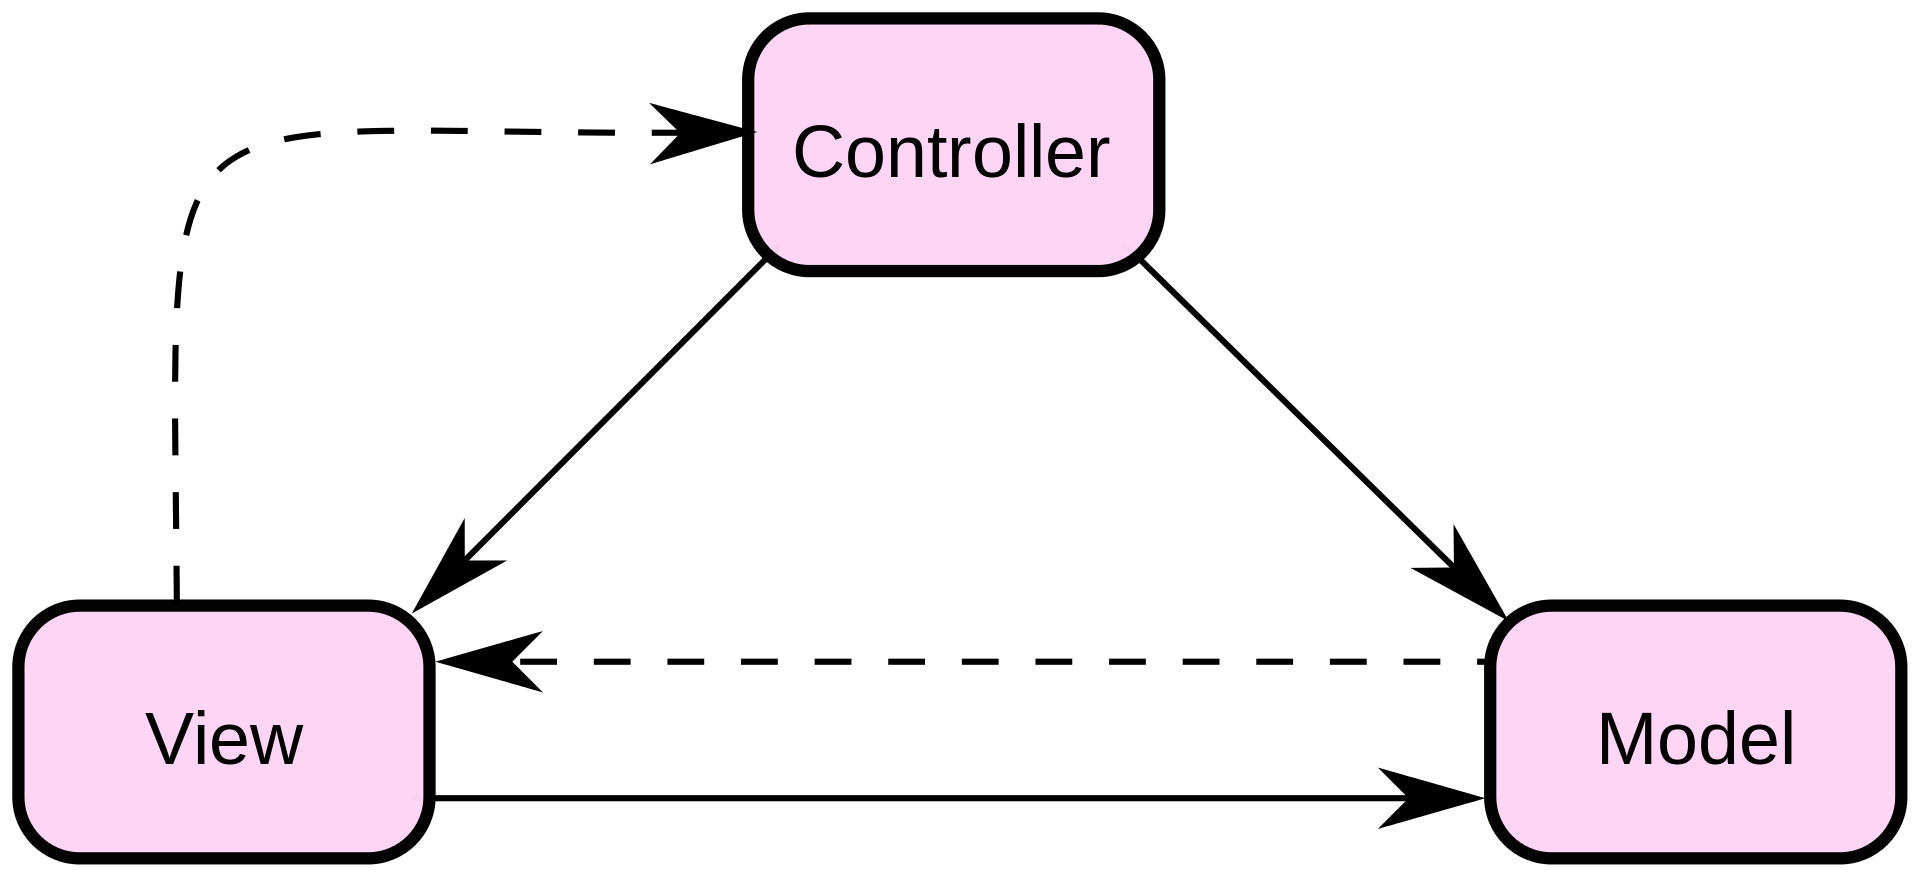
\includegraphics[width=0.5\textwidth]{figures/MVC.png}
\caption{MVC Model}
\end{figure}




\subsection{Publisher-Subscriber}
Publishers are registered on a Event Service through an Interface which let them publish Informations. There are also Subscriber which can subscribe on a Interface to receive Information. The subscriber also have to implement a Interface from the eventserver to make sure go get the information. If now a publisher publishes information the event service iterates over all possible subscriber and call a event or a function and pass the information over. 
\begin{figure}[H]
\centering
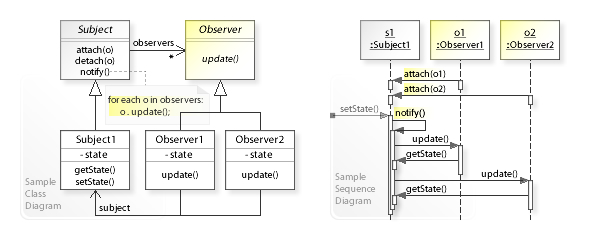
\includegraphics[width=0.5\textwidth]{figures/ObserverPrinciple.jpg}
\caption{Observer Pattern}
\end{figure}
\clearpage